\documentclass[12pt]{ctexart}
\usepackage[utf8]{inputenc}
\usepackage[T1]{fontenc}
\usepackage{graphicx}
\usepackage{xcolor}

% Other classes are available too:
% \documentclass{ctexrep}
% \documentclass{ctexbook}


\setCJKmainfont{SimSun.ttf}
\setCJKsansfont{SimHei.ttf}
\setCJKmonofont{SimFang.ttf}
%%novalidate

\usepackage{tikz}
\usepackage{calc}
\usepackage{booktabs}
%\usepackage{hyperref}

% colors
\definecolor{color1}{HTML}{000060}
%\definecolor{color1}{HTML}{8C260F}
\definecolor{color2}{HTML}{333333}


% fonts
\usepackage{fontspec}
\defaultfontfeatures{Mapping=tex-text}
\setmainfont
[BoldFont=Lato-Bold.ttf,
ItalicFont=Lato-Italic.ttf,
BoldItalicFont=Lato-BoldItalic.ttf]
{Lato-Regular.ttf}
\newfontfamily\headingfont[ItalicFont=Lato-BlackItalic.ttf]{Lato-Black.ttf}
%%%

\usepackage{geometry}
\geometry{a4paper,
hmargin=20mm,vmargin=20mm,
head=0ex,foot=3ex}

\linespread{1.3}

\usepackage[hang]{caption}
\DeclareCaptionFormat{upper}{#1#2\uppercase{#3}\par}
\captionsetup{labelfont={bf,color=color2},textfont={normalsize,color=color2},format = upper,figurename=FIGURE,tablename=TABLE}

%%% fancy sections
\usepackage{titlesec}
%\titleformat{\chapter}{\headingfont\LARGE\bfseries\scshape\color{color1}}{\thechapter}{1em}{}[\titlerule]
\titleformat{\section}{\color{color1}\headingfont\Large\bfseries\uppercase}{\thesection}{1em}{}[\titlerule]
\titleformat{\subsection}{\color{color1}\headingfont\large\bfseries\uppercase}{\thesubsection}{1em}{}
\titleformat{\subsubsection}{\color{color1}\headingfont\bfseries\uppercase}{\thesubsubsection}{1em}{}
%%%

% head and foot
\usepackage{fancyhdr}
\pagestyle{fancy}
\lhead{}
\chead{}
\makeatletter
\rhead{\color{color2}\@date}
\makeatother
\newlength{\myheight}
\lfoot{
\settoheight{\myheight}{\thepage}
\raisebox{-2ex-0.5\myheight}{
\includegraphics[height=4ex]{logo}}
}
\cfoot{\color{color2}Jing Boran 2017-04-19}
\rfoot{\color{color2}\thepage}
\renewcommand\headrulewidth{0pt}
\renewcommand\footrulewidth{0pt}

%%% picture on cover page
\usepackage{eso-pic}
\newcommand\BackgroundPic{%
\put(0,0){%
\parbox[b][\paperheight]{\paperwidth}{%
\vfill
\centering

\includegraphics[width=\paperwidth,height=\paperheight,%
keepaspectratio]{cover}%
\vfill
}}}
%%%
% custom titlepage
\makeatletter
\renewcommand{\maketitle}{
\thispagestyle{empty}
\AddToShipoutPicture*{\BackgroundPic}
\ClearShipoutPicture
%
\phantom{a}
\vfill
\phantom{a}\hfill
\begin{tabular}[c]{@{}p{0.7\textwidth}@{}}
      \color{white}\headingfont\LARGE\@title\\[1em]
      \color{white}\headingfont\Large\@author\\[2em]
\end{tabular}
%
\clearpage
}
\makeatother
%%%


%%% fancy boxes
\usepackage{tcolorbox}
\usepackage{wrapfig}
\def\fullboxbegin{
\bigskip
\begin{tcolorbox}[colback=color1,colframe=color1,coltext=white,arc=0mm,boxrule=0pt]
}
\def\fullboxend{\end{tcolorbox}\medskip}
%
\def\leftboxbegin{
\begin{wrapfigure}{l}{0.5\textwidth}
\begin{tcolorbox}[colback=color1,colframe=color1,coltext=white,arc=0mm,boxrule=0pt]
}
\def\leftboxend{
\end{tcolorbox}
\end{wrapfigure}
}
%
\def\rightboxbegin{
\begin{wrapfigure}{r}{0.5\textwidth}
\begin{tcolorbox}[colback=color1,colframe=color1,coltext=white,arc=0mm,boxrule=0pt]
}
\def\rightboxend{
\end{tcolorbox}
\end{wrapfigure}
}
%
\newcounter{frames}
\def\frameboxbegin#1{
\bigskip
\refstepcounter{frames}
\begin{tcolorbox}[colback=white,colframe=color1,arc=0mm,title={\MakeUppercase{\textbf{Frame \arabic{frames}}: #1}}]
}
\def\frameboxend{
\end{tcolorbox}
}
%%%

\usepackage{lipsum}

%%%%%%%%%%%%%%%
% Title Page
\title{井柏然 2017/04/19}
\author{BBF \newline 和你在一起 / 生日快乐!}
\date{\today}
%%%%%%%%%%%%%%%

\begin{document}
\maketitle

\tableofcontents
\clearpage

\section{序言}
\newpage

\section{你做过的事}

这是演员井柏然的成绩单。

小井在别的方面也有建树,暂时不能一一列举。

\subsection{2007-2010 BoBo组合时期}

\noindent
Cover picture filename (in titlepage): \texttt{cover}\\
Logo filename (in foot): \texttt{logo}

\subsection{Boxes}

\begin{verbatim}
\fullboxbegin
Content
\fullboxend
\end{verbatim}

\begin{verbatim}
\leftboxbegin
Content
\leftboxend
\end{verbatim}

\begin{verbatim}
\rightboxbegin
Content
\rightboxend
\end{verbatim}

\begin{verbatim}
\frameboxbegin{Frame Title}
Content
\frameboxend
\end{verbatim}

\subsection{2001-2013 重新出发}


\subsection{2004-2015 你是个演员}

\subsection{2006-今天 做更好的自己}

\newpage

\section{你说过的话}

杂志整理,访谈整理


\lipsum[1]

\fullboxbegin
\lipsum[1]
\fullboxend

\lipsum[1]
\subsection{2017-04 时装男士}
\subsection{2017-03 T风尚志}

\subsection{2016-03 南都娱乐周刊}

或许在今年之前,不少人对井柏然这个名字仍然是遥远的泛黄氤氲记忆里的选秀冠军,抑或是某些大电影中的屡屡出现的演员名字,却始终很难在第一时间把名字和脸对上号。出道八年,井柏然一度位置尴尬,尽管一直在拍电影但似乎真正的代表作不多。但在今年凭借《捉妖记》票房成功突破24亿,拍偶像剧上真人秀,人气和话题直线上 升,《三城记》《失孤》等商业文艺电影受到业内热议。井柏然迎来了自己的“井喷年”,而这也正是我们今年内第二次起用井柏然做封面的原因。

\subsubsection*{电影电视剧真人秀全面开花 —— “等”来的“井”喷年}

今年,井柏然交出的成绩着实耀眼。年初,他第一次主演偶像剧,搭档90后小花郑爽,“正经夫妇”在年轻人中曾掀起热烈的追捧。紧接着,则是真人秀《花儿与少 年》第二季中唯二男嘉宾中的一个。《捉妖记》自是不必说,《失孤》《三城记》……站在刘德华、汤唯、刘青云、秦海璐等一线实力演员身边,年轻的井柏然也并 没显得违和,在《三城记》中搭档年龄大一轮的秦海璐,也不露怯。而接下来,电影版的《盗墓笔记》也传由他出演灵魂人物张起灵,甚至电影还未开拍就引来不少的争议和讨论。
在大多数人眼中,比赛夺冠、签约华谊、唱歌演电影、顶替柯震东临时救场《捉妖记》票房大卖……一切顺风顺水,井柏然运气好得令人羡慕。
从 “以花美男选秀”著称的《加油!好男儿》出道,井柏然是当年参赛年龄最小的选手,却依靠总决赛时45万的总票数,成为了年度总冠军,一夜成名。或许是过早体验了所谓数字带来的震撼和荣耀。就算我们在采访一再提到《捉妖记》—决定他命运的《捉妖记》已早早地破了20亿票房,并朝着目前国内电影票房纪录的24.3亿日渐趋近—作为男主角的他有资格可以骄傲,“这个时候反而会让我停下来,我不是第一天在这个行业里面,周围有很多反面的教材和镜子,在这方面我一直是挺清楚的,我觉得冷静很重要。”面对井喷的成绩,26岁的井柏然依旧冷静。“我经历过一个所谓的高度,再经历过这样一个时期,我反而更清楚原来是什么样子。”井柏然用手比画了一个V形,来说明自己曾经走过的道路并不似外界想的这般顺遂。好运气同样需要蛰伏和砥砺,而这一等就是一个八年。就算是一向被冠以好资源的井柏然也经历了一个从顶点到谷底,再从谷底往上走的过程。八年似乎是好男儿们蛰伏的一个坎,在这中间离开的离开,转型的转型,而有些人则在磨亮爪牙。李易峰等待八年爆红,井柏然同样也需要一个八年来打磨自己。后选秀时代,脱离掉比赛的光环、随着组合的解散、从歌手转型拍电影,尽管井柏然一部一部拍大电影,但大多数是站在男主角边上的男二、男三。有机会主演电影,但反响似乎一般。于是渐渐地,井柏然成了“资源好到令人羡慕但成绩却总差一点”的惋惜对象,甚至关于井柏然有资源有后台的传闻不绝于耳。

在采访中,井柏然无数次提到“等待”和“坚持”。或许这成了这八年来井柏然自我安慰和拯救的鸡汤。这八年里,他耐得住性子低产地拍电影,中间有被吐槽,也有受好评的。与专注拍电视剧疯狂刷脸的演员相比,井柏然选择的道路注定更为清苦,有时候一年都拍不了几部电影,却因每部电影都是和大导演大卡司合作,即使他一部一部默默地从配角开始演起,仍然免不了招来“有后台”的质疑。在拍《失孤》的时候,沉重的电影主题和自身情绪的低潮,井柏然甚至一度怀疑自己。在这期间为了安抚躁动不已的自己,他开始每天练字让自己安静下来,摘抄的都是网络上随处可见的心灵鸡汤。以此来抵消自己的负能量和低潮期的急风骤雨。八年的等待总会有回报,今年的爆发足够让井柏然有底气证明自己,可以骄傲地说:“我的后台就是我自己。”

“一 直都能感觉到小井是比较稳健型的,虽然前几年他并没有大火,但是这几年随着他的作品越来越多,人气也越来越高,我觉得这是很理所应当的事,我相信他是那种可以持久型的,不是那种容易动荡的。”八年前《好男儿》节目组工作的K小姐曾见证井柏然的夺冠,而八年后她这样评价。

\subsubsection*{人气or作品?}

\textbf{老艺人\&新偶像的困惑}

这两年,井喷而来的青春男偶像们似乎正在迅速地接管整个娱乐圈新的节奏和话语权。影视剧也开始倾向于找他们出演,青春偶像们的片酬水涨船高,五倍十倍地翻 涨,各个商家也换上了最新最鲜的偶像代言人海报,媒体们兴奋地谈论着这一拨年轻偶像的诞生。娱乐圈似乎正在高调地进行着某种神圣的交接仪式。
偶像们正在改朝换代,偶像们正在重新分王封侯。刘德华曾经给过井柏然一个建议:要让他的海报贴满少女们的墙头,才能为自己争取到更多可能。
但在这一拨小鲜肉中,井柏然确实是一个异类。在他最新上映的电影《三城记》中,井柏然演了一名乱世中的底层工人,演对手戏的是比他年龄要整整大上一轮的秦海 璐。甚至不少人在看了海报上的名字才会把眼前这个皮肤黝黑、长满胡子一脸沧桑的“收买华”和井柏然联系在一起,哪里还有什么偶像明星、小鲜肉的样子。“我 想他也是Care颜值的,他在现场都不太照镜子,大概不愿意看到自己的样子。但他从来没有跟我抱怨过,或者提要求,反而很用心。第一天来演我就觉得他状态很对,他拉着车一嗓子吆喝,我当时一听就觉得对了,其实我并没有想过他到底怎么叫卖,可是到现场他就对了,相信他在家里肯定练过。”导演张婉婷肯定了作为偶像的井柏然的付出。
在过去的这几年,井柏然闷着头在电影在自己喜欢的质感领域里铆足了劲磨砺自己。
“我 对自己的规划和很多选择让别人觉得我像老艺人,我是保险派。”他说,“一个演员尤其是年轻艺人的寿命要更长的话,作品要对得起你自己,也不能欺骗观众。我 之前的作品都不是主角,但每一个作品拿出来我都觉得是好的东西。”那时候,他离业内更近,离少女们的墙头更远。“井柏然应该算是小鲜肉中在大电影里演技很不错的了,这也跟这么多年在电影里磨出来的结果有关。”某资深媒体人评价道。“如果他能这样继续用心去演,我相信他会前途无量,希望他不要骄傲呀。”张婉婷导演同样对井柏然颇为看好。
但井柏然不否认刘德华这句话曾给自己带来的影响,比如曾经说过不拍偶像剧的他今年拍了《相爱穿梭千年》,甚至还在团队的反复洗脑之下,上了自己曾经一度很抗拒的真人秀。偶像剧和真人秀带来的红利是显而易见的,偶像效应让井柏然被更多年轻人所熟知,无论是性格完美痴情的“公明大人”还是性格暖人逗比的导游小 井,都让井柏然的人气和话题直线上升。“至少还是在少女们的墙头贴了几张海报吧。”井柏然笑道。越来越多的人知道了井柏然,也越来越多的机会和选择纷至沓 来。
他 坦言现在有些困惑和迷茫:“我从来没觉得做配角前面就没有路,我一直都觉得特别踏实,也挺满足的。但是现在我的同事说,年轻艺人不应该闲着,也是要多拍磨炼,不要那么多的坚持。”现在的井柏然仍然时不时陷入到和团队的博弈中,作为团队自然想趁热打铁让人气再提升一个台阶,但井柏然似乎对作品角色有更多要 求。过往缓慢的节奏被日益繁忙的工作打破,这既是老艺人却又是新晋爆红的年轻偶像正在面临的选择困惑。“但是你如果真的问我的话,我还是会希望保持现在的状态,做我自己比较舒服。”井柏然想了想回答。



\subsubsection*{小井牌老好人}
\rightboxbegin

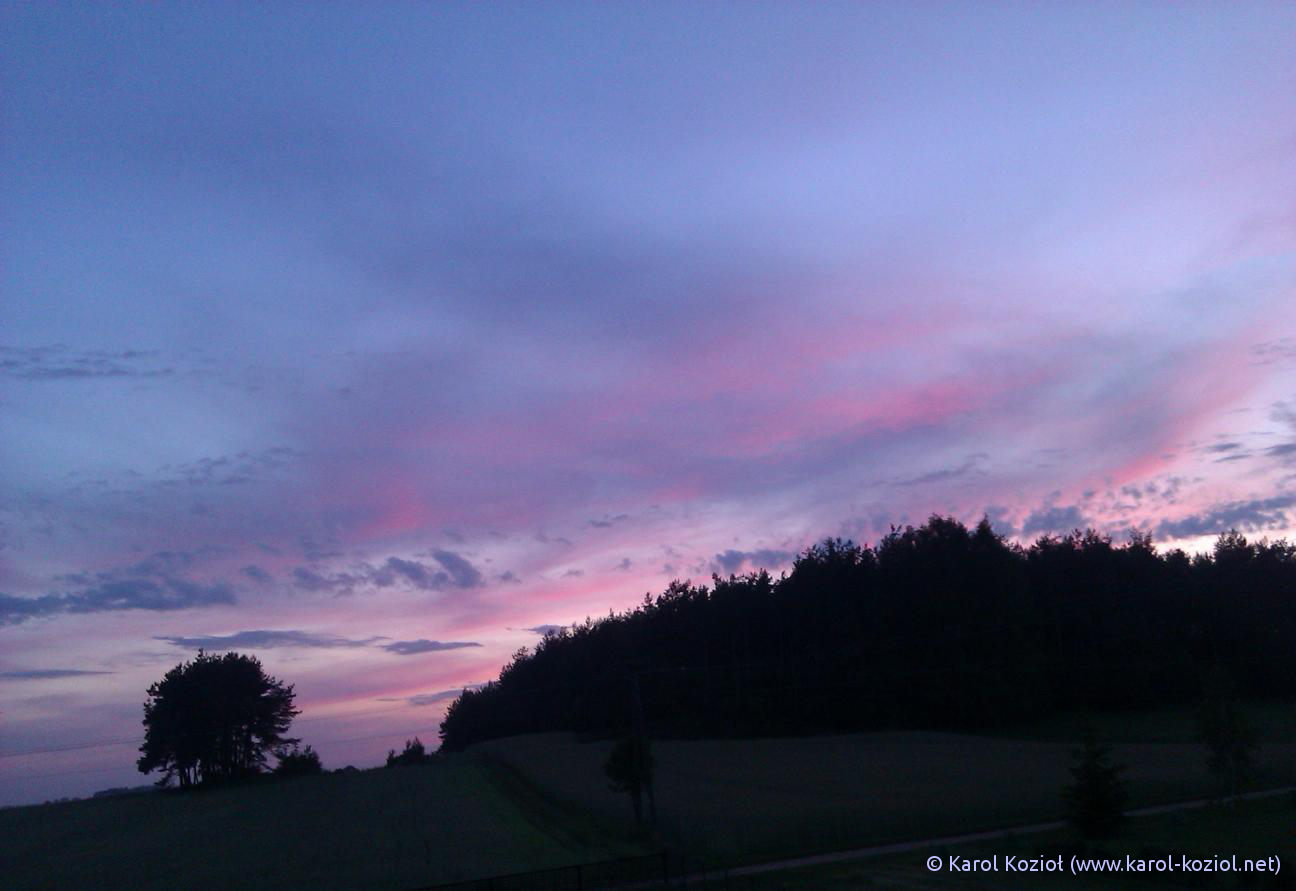
\includegraphics[width=1\textwidth]{sky.jpg}

\rightboxend
\textbf{“一旦认定了就非常认真”}



在 《花儿与少年》某一期节目中七个人徒步登山,高强度的运动量让性格直接的宁静当场就扭着脖子表示不爬了,就连郑爽也选择不干了的时候,是井柏然默默地挽着姐姐们的手,给她们加油打气成功拖着她们到了山顶。向来脾气火爆的宁静毫不讳言地夸井柏然性格脾气好、是个暖男、会照顾人。“装是很困难的,装一天、装两天、装三天,但是如果他天天都能照顾你的话,我觉得就不大像装的。”宁静在某次采访中表示。

接受本刊专访的时候,井柏然看到怀孕的记者,关心似的问这问那,并叮嘱记者要小心要注意什么事项,俨然一副过来人的样子(井柏然曾在《捉妖记》中怀孕生下胡巴)。而井柏然的好人缘似乎也和他老好人的性格分不开。由黄晓明、任泉、李冰冰开设的热辣一号,今年招收新股东,井柏然和黄渤、何炅一起新鲜入股。而他和黄晓明曾经一起出演过《血滴子》,私下两人关系也相当不错;李冰冰则是在戛纳一起走红毯熟稔起来。

自认性格慢热的井柏然,空闲的时候却喜欢宅在家里。“我是那种很难一下子真正走近你的人。如果真的是从内心真正去喜欢一个人,我觉得那个过程不会很快。如果真的喜欢一个人,我会把自己百分百丢进去,投入到一段友情或爱情中,我是那种一旦认定了就会非常认真的。”他说,“做人安分守己低调很重要。”和新生代性格张扬的偶像相比,才26岁的井柏然却有种相当沉稳的气质,说话不疾不徐,克制而不夸张,对自己的观点和逻辑都相当笃定,即使说到自己的困惑,同样也是气 场强大,是个久经历练的老艺人。所以,井柏然的朋友都是经过长时间相处的,他对于朋友也是认真付出的。曾经《好男儿》一起出道的选手中,和他关系比较好的张超提起他也是诸多夸赞。在多年后一次相遇后,两人重新恢复了联系。知道张超想重新拍戏的井柏然,介绍了一堆公司和经纪人给张超。“我以后要是上了领奖台,除了父母公司之外,最要感谢的就是井柏然。”张超说。

曾经当过《好男儿》节目宣传的Y小姐的评价似乎更为洞幽:“井柏然是个有很高的领悟力的孩子,他学东西很快,特别聪明,也因为他岁数小,特别招人疼。因为父母从小离异,跟着爷爷奶奶长大的,所以他会比较缺爱,他很喜欢有周围人的陪伴,喜欢有安全感,所以很会讨大家的欢心。而且从现在看,井柏然还是一个挺懂得感恩的人。”而他这种好人缘的积攒方法对他的事业也起到了重要作用。拍完《影子爱人》,受到导演赏识,被带到了《消失的子弹》;而和江志强合作了《黄飞鸿 之英雄有梦》,才导致在《捉妖记》需要人替补上阵的危难时刻,让江志强想到了井柏然。这种低调踏实一步步走的风格最后都得到了好的回报。



而我们没想到的是,这种克制平静的情绪在采访即将结束的尾声被打破。被问到“最想乘着时光机回到什么时候”,他的回答是爷爷奶奶年轻的时候。回想起他过世的爷爷,从小被爷爷带大的井柏然情绪明显有些波动。当他说起前一天又梦到了爷爷,悄悄地红了眼眶……这是井柏然在整段采访中唯一脆弱的时候。

\subsection{First subsection}
\subsection{First subsection}
\lipsum[1]

\leftboxbegin
Lorem ipsum dolor sit amet, consectetuer adipiscing elit. Ut purus elit, vestibulum ut, placerat ac, adipiscing vitae, felis. Curabitur dictum gravida mauris. Nam arcu libero, nonummy eget, consectetuer id, vulputate a, magna. Donec vehicula augue eu neque. 
\leftboxend

\lipsum[1-2]

\rightboxbegin
\begin{itemize}
 \item Lorem ipsum
 \item Lorem ipsum
\end{itemize}
\rightboxend

\lipsum[1]

\subsubsection{First subsubsection}

\lipsum[1]

\begin{figure}[!h]
\centering
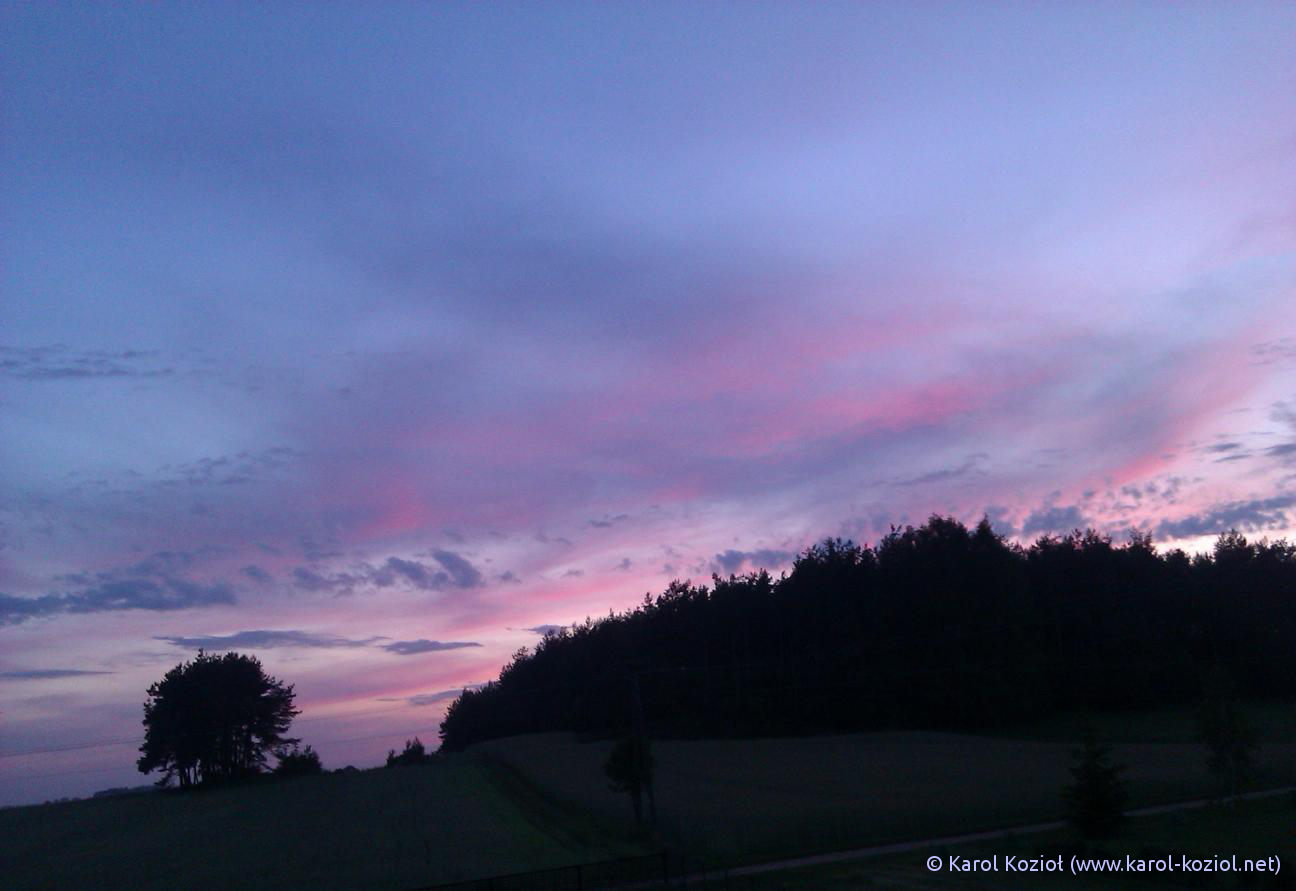
\includegraphics[width=0.5\textwidth]{sky.jpg}
\caption{The sky is the limit.}
\end{figure}

\section*{Unnumbered section}
\lipsum[1]

\begin{figure}[!h]
\centering
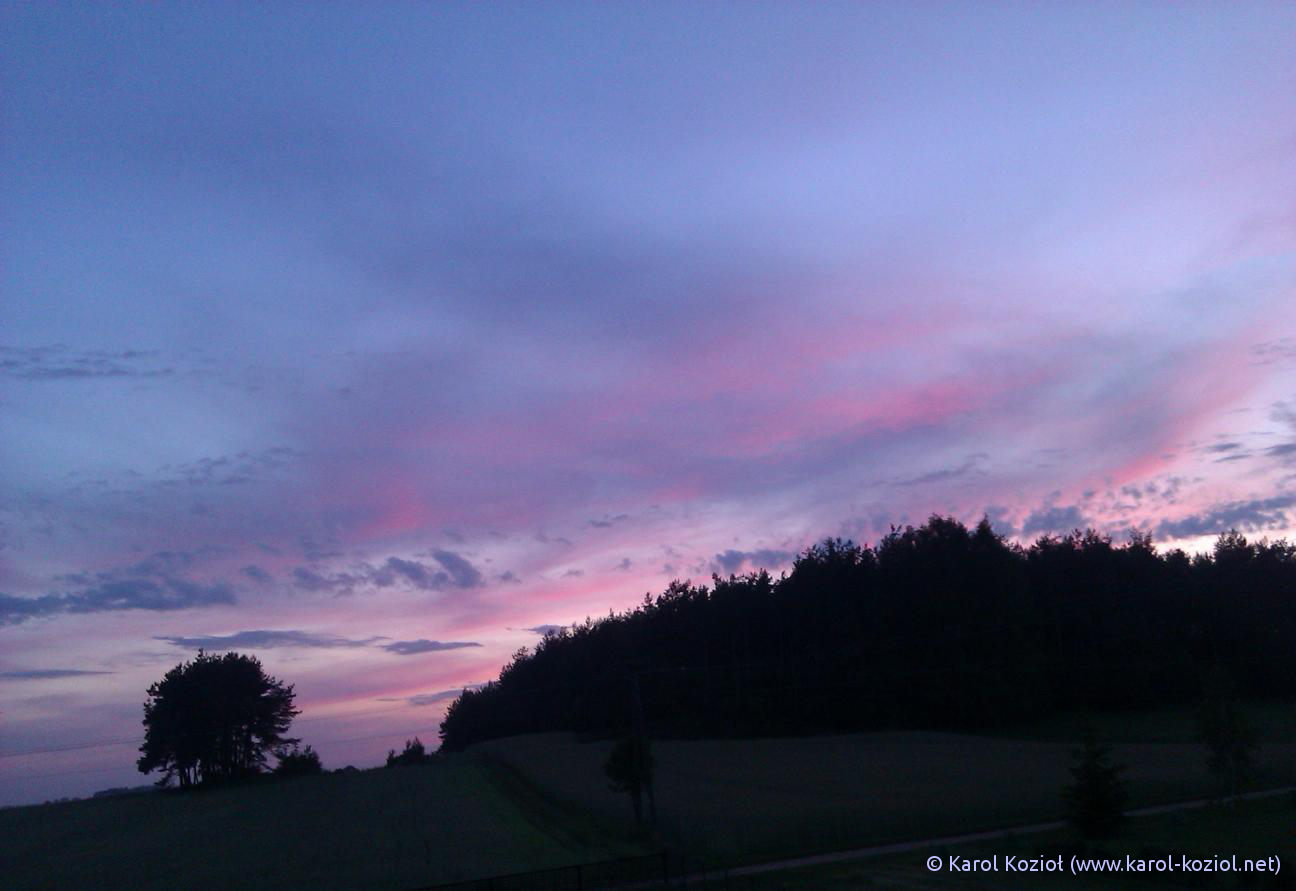
\includegraphics[width=0.5\textwidth]{sky.jpg}
\caption*{The sky is the limit.}
\end{figure}

\newpage

\section{你走过的路}

\lipsum[1]
\begin{table}[!h]
\centering
\caption{Sample table.}
\begin{tabular}{cccc}
\toprule
Value 1 & Value 2 & Value 3 & Value 4\\
\midrule
 odd     & odd   & odd & 1.00 \\
 even    & even  & even& 1.00 \\
 odd     & odd   & odd & 1.00 \\
 even    & even  & even& 1.00 \\
\bottomrule
\end{tabular}
\end{table}

\lipsum[1]

\frameboxbegin{Sample frame}
\lipsum[1]
\frameboxend
\section{送给你的祝福}

\subsection{陪你走过的十年}
\subsection{现在认识你也不晚}

\section{你的同事和朋友们}
\end{document}          
